\documentclass[10pt,a4paper]{article}

\usepackage[utf8]{inputenc}
\usepackage{amsmath,amssymb}
\usepackage{graphicx}
\usepackage{geometry}
\usepackage{array}
\usepackage{color}
\usepackage[colorlinks=true,linkcolor=blue,citecolor=blue,urlcolor=blue]{hyperref}
\usepackage{fancyhdr}
\usepackage{rotating}

% Springer LNCS text-block geometry on A4
\geometry{a4paper, textwidth=128mm, textheight=204mm, centering}

\pagestyle{fancy}
\fancyhf{}
\fancyhead[LE,RO]{\small\thepage}
\fancyhead[RE]{\small DEEPA: Dyadic-Delta Enhanced-Sheaf, Efficient Pairing with ALiBi}
\fancyhead[LO]{\small DEEPA: Hybrid Constant-State Language Modeling}
\renewcommand{\headrulewidth}{0pt}
\fancypagestyle{plain}{\fancyhf{}\renewcommand{\headrulewidth}{0pt}}

\renewcommand{\arraystretch}{1.14}
\setlength{\parindent}{1.2em}
\setlength{\parskip}{2pt}
\emergencystretch=1.5em

\newcommand{\toprule}{\hline\noalign{\smallskip}}
\newcommand{\midrule}{\noalign{\smallskip}\hline\noalign{\smallskip}}
\newcommand{\bottomrule}{\noalign{\smallskip}\hline}


% Scale a table down ONLY if it is wider than the text block (never enlarge); log its natural width.
\renewcommand{\topfraction}{0.85}\renewcommand{\bottomfraction}{0.6}\renewcommand{\textfraction}{0.12}
\renewcommand{\floatpagefraction}{0.75}\setcounter{topnumber}{3}\setcounter{totalnumber}{4}
\makeatletter
\setlength{\@fptop}{0pt}\setlength{\@fpsep}{14pt plus 2fil}\setlength{\@fpbot}{0pt plus 1fil}
\makeatother
\newsavebox{\fitb}
\newcommand{\fitwidth}[1]{\sbox{\fitb}{\setlength{\tabcolsep}{3pt}#1}\typeout{FITW \the\wd\fitb\space vs \the\textwidth}%
  \ifdim\wd\fitb>\textwidth\resizebox{\textwidth}{!}{\usebox{\fitb}}\else\usebox{\fitb}\fi}

\begin{document}
\thispagestyle{plain}

% ======================== TITLE BLOCK ========================
\begin{center}
  {\Large\bfseries DEEPA: Dyadic-Delta Enhanced-Sheaf, Efficient Pairing with ALiBi for Long-Context Language Modeling and High-Throughput Serving\par}
  \vspace{12pt}
  {\normalsize Dr.\ Deepa, Mr.\ J.\ V.\ K.\ Hem, and Mr.\ M.\ A.\ Shriram\par}
  \vspace{6pt}
  {\small\itshape Independent Researchers, Chennai, India\\
  \upshape\texttt{\char123 deepa.rME, hemjvk2004, mashriram\char125 @gmail.com}\par}
\end{center}
\vspace{6pt}

% ======================== STRUCTURED ABSTRACT (~230 words) ========================
\begin{quote}
\small
\noindent\textbf{Objectives:} Autoregressive Transformers with Rotary Position Embeddings (RoPE) incur $O(N)$ inference KV caches, quadratic $O(N^2)$ long-context training cost, and perplexity collapse beyond the training horizon. Purely recurrent models offer $O(1)$ state but degrade in exact retrieval at scale. We introduce \textbf{DEEPA} (\textbf{D}yadic-Delta \textbf{E}nhanced-sheaf, \textbf{E}fficient \textbf{P}airing with \textbf{A}LiBi), a $3:1$ hybrid sequence backbone pairing negative-eigenvalue gated delta-rule matrix memory and orthogonal dyadic sheaf diffusion with ALiBi attention.

\vspace{3pt}
\noindent\textbf{Methods:} DEEPA interleaves three \emph{Sheaf-Delta} blocks ($H_{\text{mix}}=6, d_h=64$) with one \emph{ALiBi Attention} block ($H_{\text{attn}}=8, d_a=48$) in a \texttt{dddaddda} motif. Each Sheaf-Delta layer pairs a Triton-fused chunkwise WY gated delta-rule memory ($b_t \in (0,2)$) with 5-lag isometric dyadic sheaf diffusion ($d \in \{1,2,4,8,16\}$), independent delta normalization, and SiLU output gating. Folding ALiBi biases into query/key vectors enables native FlashAttention execution (within $4\times 10^{-5}$ bpb of dense-mask loss).

\vspace{3pt}
\noindent\textbf{Results:} Across 8 byte-level domains, ALiBi-DEEPA beats Pure ALiBi on $7/8$ datasets (e.g., code $-0.047$, Hindi $-0.084$, DNA $-0.097$, Audio $-0.114$, WikiText-103 $-0.015$ bpb), leads across all four scales ($1.85\text{M}\to 38.34\text{M}$), and wins $2/3$ Long Range Arena tasks ($+12.1\%$ on 4k IMDb; ListOps tie at chance). In equal wall-clock training DEEPA beats Pure ALiBi on $3/3$ seeds ($0.7770$ vs.\ $0.7863$ bpb), and it solves parity and $S_3$ state tracking where attention baselines fail (a $\beta\in(0,1)$ control confirms negative eigenvalues are responsible). It extrapolates monotonically to $16\text{k}$ ($1.507\to 1.469$ vs.\ RoPE $5.299$), cuts KV cache by $4\times$, increases 8 GB serving throughput by $3.7\text{--}4.8\times$ vs.\ RoPE ($3.1\text{--}4.2\times$ vs.\ ALiBi), and trains $1.16\text{--}1.57\times$ faster than RoPE ($1.06\text{--}1.46\times$ faster than folded ALiBi) at $4\text{k}\text{--}16\text{k}$.

\vspace{3pt}
\noindent\textbf{Conclusion:} DEEPA delivers competitive or superior modeling quality across modalities alongside $4\times$ smaller KV caches, stable $16\times$ extrapolation, and higher long-context throughput, while documenting its limits at short contexts ($T\le 1\text{k}$) and fixed 2D raster strides.

\vspace{4pt}
\noindent\textbf{Keywords:} Hybrid Sequence Modeling, Gated Delta Rule, Dyadic Sheaf Diffusion, ALiBi, FlashAttention, Length Extrapolation, Constant-State Decoding.
\end{quote}

\vspace{4pt}

% ======================== SECTION 1 ========================
\section{Introduction}

Autoregressive Transformers \cite{vaswani2017} paired with Rotary Position Embeddings (RoPE) \cite{su2024} form the backbone of modern language models, yet impose three structural bottlenecks in long-context and resource-constrained settings: (1) an $O(N)$ per-sequence Key-Value (KV) cache across all $L$ layers that caps concurrent serving batch size and makes decoding memory-bandwidth bound; (2) quadratic $O(N^2 D)$ training and prefill scaling; and (3) catastrophic out-of-distribution perplexity degradation when evaluating beyond the training horizon $N_{\text{train}}$.

Purely recurrent architectures---including linear attention \cite{katharopoulos2020}, selective state-space models (Mamba-1/2) \cite{gu2023,dao2024}, and fast-weight delta networks \cite{schlag2021,yang2024b,yang2024c}---replace the $O(N)$ KV cache with a fixed-size state. However, positive-gated diagonal recurrences cannot track parity (which requires a negative eigenvalue) or non-abelian groups such as $S_3$ \cite{merrill2024,grazzi2024}, and purely recurrent models often lag full attention on exact in-context retrieval as capacity grows. Hybrid backbones such as Jamba \cite{lieber2024} and Samba \cite{ren2024} interleave recurrent and attention layers, yet typically combine positive-eigenvalue diagonal SSMs with RoPE or sliding-window attention, retaining either RoPE's length collapse or truncated context windows.

We introduce \textbf{DEEPA} (\textbf{D}yadic-Delta \textbf{E}nhanced-sheaf, \textbf{E}fficient \textbf{P}airing with \textbf{A}LiBi), a $3:1$ hybrid architecture (\texttt{dddaddda}) that pairs three \emph{Sheaf-Delta} blocks with one \emph{ALiBi Attention} block. Every design choice in DEEPA is validated through multi-seed ablations, exact forward/step equivalence checks, and cross-modal evaluation.

\subsection{Key Contributions}
\begin{enumerate}
  \item \textbf{Distinctive Hybrid Mechanism:} DEEPA combines negative-eigenvalue gated delta-rule matrix memory ($b_t \in (0,2)$) \cite{grazzi2024} with a parallel, isometric multi-scale causal dyadic sheaf diffusion path ($d \in \{1,2,4,8,16\}$) and unrotated ALiBi attention \cite{press2022} in a $3:1$ ratio (the best among the ratios tested: $3:1$ vs.\ $4:1$ and pure baselines). Unlike Jamba, Samba, or standard Gated DeltaNet, DEEPA operates without a causal $q,k$ token-shift/convolution mixer (we show a causal $q,k$ token shift degrades delta-rule erasure by $+0.046$ bpb) and preserves unrotated shift-invariant feature coordinates across recurrent and attention layers.
  \item \textbf{FlashAttention-Compatible ALiBi Folding \& Compiler Fusion:} By folding ALiBi's linear distance bias directly into query/key vectors (exact to $4\times 10^{-5}$ bpb), combining Triton chunkwise WY delta kernels with zero-copy dyadic slices, and applying whole-model \texttt{torch.compile}, DEEPA trains $1.16\text{--}1.57\times$ faster than FlashAttention RoPE GPT ($1.06\text{--}1.46\times$ faster than folded-kernel Pure ALiBi) from $4\text{k}$ to $16\text{k}$, cuts inference KV cache by $4\times$, and boosts 8 GB serving throughput by $3.7\text{--}4.8\times$ vs.\ RoPE GPT ($3.1\text{--}4.2\times$ vs.\ Pure ALiBi).
  \item \textbf{Multi-Modal, Scaling, Extrapolation, and Mechanism Evaluation:} Across 8 real-world domains (enwik8 \cite{hutter2006}, WikiText-103 \cite{merity2016}, Python code \cite{codeparrot}, Hindi, Chinese, DNA \cite{grch38}, CIFAR-10 pixels \cite{krizhevsky2009}, 16 kHz $\mu$-law audio \cite{warden2018,vandenoord2016}), 4 scales ($1.85\text{M}\to 38.34\text{M}$ at matched $5$ tokens/param), 18,000-step Chinchilla-ratio convergence \cite{hoffmann2022}, 3-seed $16\times$ extrapolation, Long Range Arena \cite{tay2021}, and a 9-task converged synthetic suite, DEEPA establishes strong quality and efficiency gains alongside clearly defined boundaries.
\end{enumerate}

% ======================== SECTION 2 ========================
\section{Related Work and Positioning Against Existing Hybrids}

\subsection{Gated Delta Rules and Negative-Eigenvalue Transitions}
Linear attention \cite{katharopoulos2020} compresses history into an additive matrix $S_t = \sum_{i\le t} v_i k_i^\top$, which saturates on long sequences. DeltaNet \cite{schlag2021,yang2024b} and Gated DeltaNet \cite{yang2024c} introduce selective key erasure via the Widrow-Hoff delta rule and scalar exponential decay, parallelized via the compact WY representation \cite{bischof1987}. Grazzi et al.\ \cite{grazzi2024} showed that expanding the step size $\beta_t$ from $(0,1)$ to $(0,2)$ enables negative eigenvalues ($\lambda=-1$ at $\beta_t=2$, exact Householder reflections), unlocking parity and finite-state tracking that diagonal positive-gated SSMs (Mamba-1/2 \cite{gu2023,dao2024}) cannot express \cite{merrill2024}. Siems et al.\ \cite{siems2025} further generalized single-step reflections to multi-reflection products.

\subsection{Hybrid Recurrent-Attention Architectures and Length Extrapolation}
Hybrid models such as Jamba ($7:1$ Mamba:Attention) \cite{lieber2024}, Samba ($1:1$ Mamba:Sliding-Window Attention) \cite{ren2024}, and Mamba-2 Hybrid \cite{waleffe2024} show that interleaving a small fraction of attention layers recovers exact retrieval while preserving recurrent efficiency. Separately, length extrapolation in Transformers has been studied via ALiBi \cite{press2022}, NoPE \cite{kazemnejad2023}, and RoPE frequency rescaling (YaRN \cite{peng2023}).

\subsection{How DEEPA Differs from Existing Hybrid Transformers}
Table~\ref{tab:taxonomy} contrasts DEEPA against four representative families across six structural axes.

\begin{table}[htbp]
\centering
\caption{Architectural taxonomy contrasting DEEPA against existing hybrid and recurrent backbones across six design axes.}
\label{tab:taxonomy}
\fitwidth{%
\begin{tabular}{>{\raggedright\arraybackslash}p{2.1cm}>{\raggedright\arraybackslash}p{2.2cm}>{\raggedright\arraybackslash}p{2.3cm}>{\raggedright\arraybackslash}p{1.7cm}>{\raggedright\arraybackslash}p{1.6cm}>{\raggedright\arraybackslash}p{2.0cm}}
\toprule
\textbf{Architecture} & \textbf{Recurrent State Eigenvalues} & \textbf{Local Context Path} & \textbf{Attn Ratio / Type} & \textbf{Pos.\ Encoding} & \textbf{Decode State / $16\times$ Extrap.} \\
\midrule
\textbf{RoPE GPT} \cite{su2024} & None & Full Attention & $0:1$ Full & RoPE (rotates $q,k$) & $O(L N)$ / Collapses \\
\textbf{Pure ALiBi} \cite{press2022} & None & Full Attention & $0:1$ Full & ALiBi (unrotated) & $O(L N)$ / Stable \\
\textbf{Jamba} \cite{lieber2024} & Diagonal $\lambda \in (0,1)$ (Mamba) & Depthwise Conv1d ($k=4$) & $7:1$ Full & RoPE & $\frac{1}{8}O(LN)$ / RoPE-bound \\
\textbf{Samba} \cite{ren2024} & Diagonal $\lambda \in (0,1)$ (Mamba) & Depthwise Conv1d ($k=4$) & $1:1$ SWA & RoPE + Window & $O(LW)$ / Window-bound \\
\textbf{Gated DeltaNet} \cite{yang2024c} & Projection $\lambda \in [0,1]$ ($\beta \in (0,1)$) & Short Conv1d on $q,k,v$ & Pure Rec.\ (no attn) & None & $O(L d_h^2)$ / Retrieval-limited \\
\textbf{DEEPA (Ours)} & \textbf{Reflection $\lambda \in [-1,1]$} & \textbf{Parallel Dyadic Sheaf ($d \in \{1..16\}$, $U^\top U=I$)} & \textbf{$3:1$ Full (\texttt{dddaddda})} & \textbf{Flash-folded ALiBi} & \textbf{$\frac{1}{4}O(LN)$ / Stable $16\times$} \\
\bottomrule
\end{tabular}}
\end{table}

\noindent\textbf{Discussion of Table~\ref{tab:taxonomy}:} DEEPA introduces three coupled departures from existing hybrids: (i) unlike Jamba, Samba, and standard Gated DeltaNet ($\beta \in (0,1)$, $\lambda \in [0,1]$), its recurrent layers adopt Grazzi et al.'s \cite{grazzi2024} $\beta_t \in (0,2)$ reflection regime ($\lambda \in [-1,1]$) required for parity and $S_3$ state tracking; (ii) unlike Gated DeltaNet and Mamba, DEEPA replaces local $q,k$ filtering with a \emph{parallel}, norm-preserving multi-scale dyadic sheaf transport at exponentially spaced lags $\{1,2,4,8,16\}$ (Section~\ref{sec:ablation} shows that a causal $q,k$ token shift---a convolution-like local mixer---degrades DEEPA by $+0.046$ bpb by making consecutive unit keys collinear); and (iii) pairing unrotated Sheaf-Delta stalks with FlashAttention-folded ALiBi avoids RoPE's coordinate rotation mismatch while preserving full global attention in $25\%$ of layers rather than truncating via sliding windows.

% ======================== SECTION 3 ========================
\section{The DEEPA Architecture and Mathematical Formulation}

Table~\ref{tab:notation} defines every symbol and tensor shape used throughout this section.

\begin{table}[htbp]
\centering
\caption{Complete notation and symbol glossary for DEEPA (default $14.44\text{M}$ \texttt{h6} configuration: $D=384, L=8, H_{\text{mix}}=6, d_h=64, H_{\text{attn}}=8, d_a=48$).}
\label{tab:notation}
\fitwidth{%
\begin{tabular}{>{\raggedright\arraybackslash}p{1.8cm}>{\raggedright\arraybackslash}p{2.5cm}>{\raggedright\arraybackslash}p{7.8cm}}
\toprule
\textbf{Symbol} & \textbf{Shape / Domain} & \textbf{Definition and Role} \\
\midrule
$B, T, D$ & $\mathbb{N}$ & Batch size, sequence length, and model hidden dimension ($D=384$). \\
$L, \mathcal{P}$ & $L=8$, \texttt{dddaddda} & Total blocks and repeating $3:1$ layer pattern (\texttt{d}=Sheaf-Delta, \texttt{a}=ALiBi). \\
$H_{\text{mix}}, d_h$ & $6, 64$ & Number of Sheaf-Delta mixer heads and per-head dimension ($H_{\text{mix}} d_h = D$). \\
$H_{\text{attn}}, d_a$ & $8, 48$ & Number of ALiBi attention heads and per-head dimension ($H_{\text{attn}} d_a = D$). \\
$x_t \in \mathbb{R}^D$ & $[B, T, D]$ & Pre-RMSNorm residual stream representation (stalk) at token position $t$. \\
$\hat{q}_t, \hat{k}_t, v_t$ & $[B, H_{\text{mix}}, T, d_h]$ & L2-normalized query/key vectors ($\|\hat{q}_t\|_2=\|\hat{k}_t\|_2=1$) and value vector. \\
$S_t$ & $[B, H_{\text{mix}}, d_h, d_h]$ & Per-head associative matrix memory (``notebook'' state) at step $t$. \\
$a_t, b_t$ & $(0.8, 1)$, $(0, 2)$ & Per-head scalar retention decay gate and Householder erasure/write step size. \\
$\mathcal{D}, d$ & $\{1, 2, 4, 8, 16\}$ & Exponentially spaced causal dyadic lags for local sheaf transport. \\
$U_{t,d}$ & $d_h \times d_h$ ($U^\top U=I$) & Orthogonal transport map formed by $M=2$ thin Householder reflections. \\
$g_{t,d}$ & $(0, 1)$ & Learned sigmoid edge gate weighting transported message from position $t-d$. \\
$o_t^{\text{delta}}, o_t^{\text{dyadic}}$ & $[B, H_{\text{mix}}, T, d_h]$ & Outputs of the global delta-rule branch and local dyadic sheaf branch. \\
$m_h$ & $2^{-8h/H_{\text{attn}}}$ & Fixed geometric ALiBi slope for attention head $h \in \{1,\dots,H_{\text{attn}}\}$. \\
\bottomrule
\end{tabular}}
\end{table}

\subsection{Macro $3:1$ Topology and Information Flow}
Figure~\ref{fig:arch} illustrates both the macro 8-layer \texttt{dddaddda} backbone and the internal micro-dataflow of the Sheaf-Delta (\texttt{d}) and ALiBi Attention (\texttt{a}) blocks.

\begin{figure}[htbp]
  \centering
  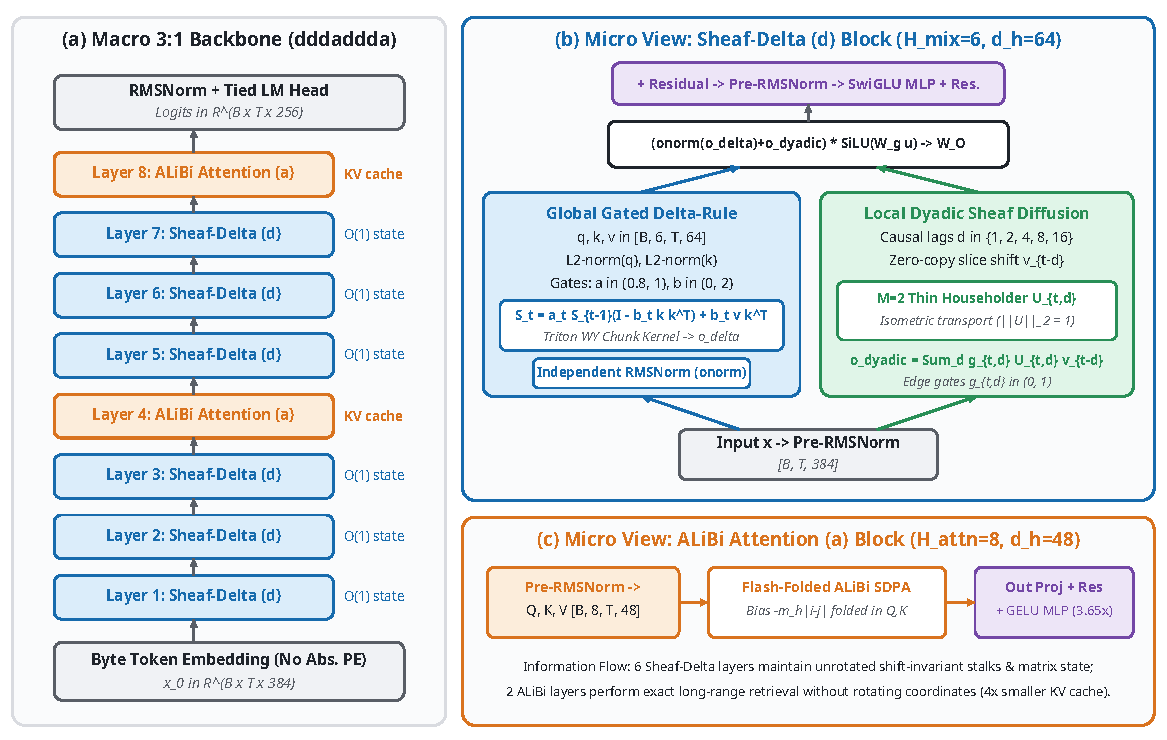
\includegraphics[width=\textwidth]{figs/fig1_architecture.pdf}
  \caption{DEEPA $3:1$ architecture and information flow. \textbf{(a)} Macro 8-layer \texttt{dddaddda} stack: six Sheaf-Delta layers maintain $O(1)$ recurrent state while two ALiBi layers maintain KV caches ($4\times$ smaller total cache). \textbf{(b)} Micro Sheaf-Delta block splitting into parallel Global Gated Delta-Rule and Local Dyadic Sheaf branches with independent \texttt{onorm} and SiLU output gating. \textbf{(c)} Micro ALiBi Attention block with FlashAttention-folded distance biases and GELU MLP.}
  \label{fig:arch}
\end{figure}

\noindent\textbf{Step-by-Step Information Flow:} Raw byte tokens ($V=256$) are embedded into $x_0 \in \mathbb{R}^{B \times T \times 384}$ with \emph{no absolute positional embedding}. Every block $\ell \in \{1,\dots,L\}$ applies pre-RMSNorm residual updates:
\begin{equation}
  h_\ell = x_{\ell-1} + \text{Mixer}_\ell(\text{RMSNorm}(x_{\ell-1})), \qquad
  x_\ell = h_\ell + \text{MLP}_\ell(\text{RMSNorm}(h_\ell)),
  \label{eq:residual}
\end{equation}
where Sheaf-Delta blocks (\texttt{d}) use a SwiGLU MLP (\texttt{mlp\_mult}=3.65), ALiBi Attention blocks (\texttt{a}) inside DEEPA use a two-layer GELU MLP (\texttt{mlp\_mult}=3.65), and the Pure ALiBi and RoPE GPT baselines use a standard two-layer GELU MLP (\texttt{mlp\_mult}=4.0) to match parameter budgets.

In Layers 1--3 (\texttt{d}), each Sheaf-Delta block reshapes the normalized input into $[B, 6, T, 64]$ ($d_h=64$ aligns directly with Triton's $64\times 64$ Tensor Core tiles), aggregates local multi-scale context via dyadic lags $\{1,2,4,8,16\}$ while updating its fixed $64\times 64$ global matrix memory, and projects back to $[B, T, 384]$. Because no positional rotation is applied, these three layers produce shift-invariant, locally contextualized features. Layer 4 (\texttt{a}) then reshapes $[B, T, 384] \to [B, 8, T, 48]$ and performs exact all-pairs causal retrieval via Flash-folded ALiBi attention without rotating feature coordinates. Layers 5--7 (\texttt{d}) refine the retrieved representations over long horizons, and Layer 8 (\texttt{a}) performs a final global retrieval pass before the tied LM head produces logits in $\mathbb{R}^{B \times T \times 256}$.

\subsection{Branch 1: Global Gated Delta-Rule Matrix Memory}
For each mixer head $h \in \{1,\dots,H_{\text{mix}}\}$, linear projections map $u_t = \text{RMSNorm}(x_t)$ to $q_t, k_t, v_t \in \mathbb{R}^{d_h}$ and two scalar gate logits $(z_{b,t}, z_{a,t})$:
\begin{equation}
  \begin{aligned}
  \hat{q}_t &= \frac{q_t}{\|q_t\|_2 + \epsilon}, \qquad
  \hat{k}_t = \frac{k_t}{\|k_t\|_2 + \epsilon}, \\
  b_t &= 2\sigma(z_{b,t}) \in (0, 2), \qquad
  a_t = 0.8 + 0.2\sigma(z_{a,t}) \in (0.8, 1).
  \end{aligned}
  \label{eq:gates}
\end{equation}
The decay bias $z_{a,t}$ is initialized to $+3.0$, setting the initial retention rate to $a_0 \approx 0.9905$ (a $\sim 73$-token half-life). The matrix memory $S_t \in \mathbb{R}^{d_h \times d_h}$ updates and reads out as:
\begin{equation}
  S_t = a_t S_{t-1}\!\left(I - b_t \hat{k}_t \hat{k}_t^\top\right) + b_t v_t \hat{k}_t^\top, \qquad
  o_t^{\text{delta}} = d_h^{-1/2}\, S_t \hat{q}_t.
  \label{eq:delta}
\end{equation}
\noindent\textbf{Intuition \& Role of Each Term:} Think of $S_t$ as a fixed-size associative ``notebook'' storing key-value bindings. First, $a_t \in (0.8,1)$ gently fades older entries globally. Second, $(I - b_t \hat{k}_t \hat{k}_t^\top)$ selectively erases or reflects whatever was previously stored under key $\hat{k}_t$: at $b_t=1$ it projects out the old value cleanly before writing $v_t \hat{k}_t^\top$; at $b_t=2$ it becomes an exact Householder reflection ($\lambda = -1$ along $\hat{k}_t$), allowing the state to flip sign and track parity ($\mathbb{Z}_2$) and non-abelian group states such as $S_3$ over arbitrary lengths \cite{grazzi2024}. L2-normalizing $\hat{k}_t$ guarantees the spectral norm $\|I - b_t \hat{k}_t \hat{k}_t^\top\|_2 \le 1$, preventing state explosion. During training, Eq.~\eqref{eq:delta} is evaluated in parallel chunks via the Triton WY kernel \texttt{chunk\_gated\_delta\_rule}; during decoding, it executes in $O(d_h^2)$ time with a constant $61.4\text{ KB}$ bf16 state per layer ($30{,}720$ values including the 16-token dyadic ring buffer).

\subsection{Branch 2: Parallel Multi-Scale Causal Dyadic Sheaf Diffusion}
Running in parallel with Eq.~\eqref{eq:delta}, the dyadic sheaf branch transports value vectors $v_{t-d}$ from five exponentially spaced causal lags $d \in \mathcal{D} = \{1, 2, 4, 8, 16\}$ into the current stalk at position $t$:
\begin{equation}
  U_{t,d} = \prod_{m=1}^{2}\!\left(I - 2\,\hat{r}_{d,m}\hat{r}_{d,m}^\top\right), \qquad
  o_t^{\text{dyadic}} = \sum_{d \in \mathcal{D}} g_{t,d}\, U_{t,d}\, v_{t-d},
  \label{eq:dyadic}
\end{equation}
where $\hat{r}_{d,m} \in \mathbb{R}^{d_h}$ are L2-normalized learned reflector vectors (orthogonal transport $U_{t,d}^\top U_{t,d} = I$) and $g_{t,d} = \sigma(w_d^\top u_t + c_d) \in (0,1)$ are input-dependent edge gates.

\noindent\textbf{Intuition \& Role of Each Term:} While the delta notebook $S_t$ tracks global compressed state, local byte-level syntax (multi-byte UTF-8 characters, code indentation, DNA motifs, audio oscillations) benefits from distortion-free local aggregation. Applying $M=2$ Householder reflections costs only $O(d_h)$ vector dot products (never materializing a $d_h \times d_h$ matrix) and is strictly \emph{isometric} ($\|U_{t,d} v_{t-d}\|_2 = \|v_{t-d}\|_2$), rotating neighboring token features into the current coordinate frame without amplifying or vanishing gradients. Using zero-copy tensor slices (\texttt{v[:, :, :-d, :]}) eliminates 2D index-gather overhead during training and uses a fixed 16-token ring buffer during decoding.

\subsection{Branch Fusion, Output Gating, and Flash-Folded ALiBi}
The two branches are fused via \emph{independent} pre-sum normalization of the delta branch followed by a learned SiLU output gate:
\begin{equation}
  y_t = W_O \Big[\big(\text{RMSNorm}_{\text{delta}}(o_t^{\text{delta}}) + o_t^{\text{dyadic}}\big) \odot \text{SiLU}(W_g u_t)\Big].
  \label{eq:fuse}
\end{equation}
\noindent\textbf{Intuition:} The delta readout $o_t^{\text{delta}} = d_h^{-1/2} S_t \hat{q}_t$ has state-norm-dependent scale, whereas $o_t^{\text{dyadic}}$ is already an isometric transport modulated by bounded gates $g_{t,d} \in (0,1)$. Normalizing $o_t^{\text{delta}}$ independently prevents bursts of local dyadic activity from rescaling global memory (confirmed in Table~\ref{tab:ablation}, where post-sum normalization degrades loss by $+0.030$ to $+0.044$ bpb), while $\text{SiLU}(W_g u_t)$ provides input-dependent channel gating prior to $W_O$.

In the two attention layers (\texttt{a}), ALiBi adds a linear distance bias $-m_h (i - j)$ ($i \ge j$) to attention logits \cite{press2022}. Passing an explicit $[H, T, T]$ bias matrix disables FlashAttention \cite{dao2022} and requires $8.6\text{ GB}$ at $T=16,384$. Because $-m_h (i - j) = (-m_h i)\cdot 1 + 1\cdot(m_h j)$ is a rank-2 inner product, we fold the exact linear bias into augmented query/key coordinates (padded to FlashAttention's supported head dimension), executing ALiBi natively inside FlashAttention. Across validation checks, this folded kernel matches dense-mask ALiBi to within $4\times 10^{-5}$ bpb while yielding measured training speedups of $1.13\text{--}1.89\times$ from $2\text{k}$ to $16\text{k}$ for DEEPA ($0.90\times$ at $1\text{k}$ due to padding overhead) and $1.24\text{--}3.6\times$ for Pure ALiBi.

\subsection{Computational Overhead and Memory Complexity}
Table~\ref{tab:complexity} summarizes the closed-form training and inference complexity of DEEPA relative to full-attention Transformers.

\begin{table}[htbp]
\centering
\caption{Analytical computational and memory complexity ($14.4\text{M}$ models, $D=384, L=8, H_{\text{mix}}=6, d_h=64$, bf16 cache).}
\label{tab:complexity}
\fitwidth{%
\begin{tabular}{lccccc}
\toprule
\textbf{Model} & \textbf{Train Time} & \textbf{Decode Step} & \textbf{Cache Formula (bf16 vals)} & \textbf{Cache @16k} & \textbf{Cache @65k} \\
\midrule
\textbf{Pure ALiBi / RoPE} & $O(L T D^2 + L T^2 D)$ & $O(L D^2 + L T D)$ & $8 \times (2 T D)$ & $201.3\text{ MB}$ & $805.3\text{ MB}$ \\
\textbf{ALiBi-DEEPA 3:1} & $O(L T D^2 + \frac{L}{4} T^2 D)$ & $O(L D^2 + \frac{L}{4} T D)$ & $6 \times 30{,}720 + 2 \times (2 T D)$ & \textbf{$50.7\text{ MB}$} & \textbf{$201.7\text{ MB}$} \\
\textbf{Pure SheafDelta} & $O(L T D^2 + L T D d_h)$ & $O(L D^2 + L D d_h)$ & $8 \times 30{,}720$ (const.) & \textbf{$0.49\text{ MB}$} & \textbf{$0.49\text{ MB}$} \\
\bottomrule
\end{tabular}}
\end{table}

\noindent\textbf{Discussion of Table~\ref{tab:complexity}:} Each Sheaf-Delta layer stores $H_{\text{mix}} d_h^2 + 16 D = 30{,}720$ bf16 values ($61.4\text{ KB}$ per sequence, independent of $T$). Consequently, ALiBi-DEEPA reduces the quadratic attention term and linear KV cache by $4\times$ at every length ($50.7$ vs.\ $201.3\text{ MB}$ at $16\text{k}$; $201.7$ vs.\ $805.3\text{ MB}$ at $65\text{k}$). The main training overhead of DEEPA is WY-chunk intermediate storage and small-kernel launch latency in the 6 Sheaf-Delta layers, which increases peak training VRAM by $14\%$ vs.\ RoPE GPT ($20\%$ vs.\ folded-kernel Pure ALiBi) at $16\text{k}$ and slows short-context ($T\le 1\text{k}$) steps before the crossover between $2\text{k}$ and $4\text{k}$ (Section~\ref{sec:systems}).

% ======================== SECTION 4 ========================
\section{Experimental Protocol}

All primary experiments run on a single NVIDIA RTX 2000 Ada Laptop GPU ($8\text{ GB}$ VRAM) in \texttt{bfloat16} with \texttt{torch.compile}. Unless noted, models follow our $14.4\text{M}$-parameter byte-level recipe ($V=256, D=384, L=8$; SwiGLU \texttt{mlp\_mult}=3.65 in Sheaf-Delta blocks, GELU \texttt{mlp\_mult}=3.65 in DEEPA's attention blocks, and GELU \texttt{mlp\_mult}=4.0 in the Pure ALiBi and RoPE GPT baselines; AdamW $\beta=(0.9,0.95)$, uniform weight decay $0.05$, peak LR $2\times 10^{-3}$, 100-step linear warmup, cosine decay to $0.1\times$, gradient clip $1.0$, batch $B=16$, context $T=1024$). ALiBi-DEEPA 3:1 (\texttt{h6}) has $14,436,348$ parameters; Pure ALiBi and RoPE GPT have $14,260,608$ parameters. All multi-seed standard deviations use population std ($\text{ddof}=0$) consistently across every table, and all bpb differences follow a unified sign convention where \textbf{negative $\Delta$ bpb indicates lower loss (better)}.

\noindent\textbf{Evaluation-Slice Disclosure:} Early benchmarks on \texttt{enwik8} scored the first $64$ windows $\times 1024 = 64\text{ KB}$ of the $1\text{ MB}$ validation slice (\texttt{val\_bpb}), which is easier than later blocks ($1.02$ vs.\ $1.21\text{--}1.90$ bpb). Relative comparisons on identical windows remain valid, and all multi-domain, scaling, and extrapolation tables report the \textbf{full 1 MB validation set} ($976$ windows) or a fixed $512\text{ KB}$ budget shared identically across lengths.

% ======================== SECTION 5 ========================
\section{Experimental Results}

\subsection{Chinchilla-Ratio Convergence and Equal Wall-Clock on enwik8}
To test whether DEEPA's early-training advantage persists at longer training horizons, Table~\ref{tab:chinchilla} compares ALiBi-DEEPA 3:1 (\texttt{h6}) against Pure ALiBi over $18,000$ steps ($294.9\text{M}$ tokens $\approx 20.4$ tokens/param, $7.4$ repeated epochs over the $40\text{ MB}$ \texttt{enwik8} slice) across 3 seeds, together with an equal-wall-clock $13{,}300$-step DEEPA run and the 1,500-step uniform vs.\ split weight-decay check.

\begin{table}[htbp]
\centering
\caption{3-seed Chinchilla-ratio convergence \cite{hoffmann2022} ($18,000$ steps, $\approx 20.4$ tokens/param, $7.4$ repeated epochs over $40\text{ MB}$ \texttt{enwik8}), equal folded-kernel wall-clock ($13{,}300$ steps), and weight-decay ablation ($1,500$ steps; 64 KB validation slice, mean $\pm$ population std).}
\label{tab:chinchilla}
\fitwidth{%
\begin{tabular}{lcccccc}
\toprule
\textbf{Experiment / Model (3 seeds)} & \textbf{Steps} & \textbf{Val @1024} & \textbf{Per-Seed @1024} & \textbf{@2048} & \textbf{@4096} & \textbf{tok/s$^*$} \\
\midrule
\textbf{18k: ALiBi-DEEPA 3:1 (h6)} & 18,000 & \textbf{0.7794 $\pm$ .0025} & \textbf{.7820/.7761/.7801} & \textbf{0.7620 $\pm$ .0021} & \textbf{0.8246 $\pm$ .0034} & 80.6k \\
\textbf{13.3k (Iso-Time): DEEPA (h6)} & 13,300 & \textbf{0.7770 $\pm$ .0010} & \textbf{.7776/.7756/.7779} & \textbf{0.7585 $\pm$ .0012} & \textbf{0.8183 $\pm$ .0021} & 80.9k \\
\textbf{18k: Pure ALiBi} & 18,000 & 0.7863 $\pm$ .0049 & .7924/.7861/.7803 & 0.7664 $\pm$ .0047 & 0.8258 $\pm$ .0041 & 85.3k \\
\textbf{13.3k (Equal-Steps): Pure ALiBi} & 13,300 & 0.7888 $\pm$ .0029 & .7891/.7851/.7921 & 0.7688 $\pm$ .0021 & 0.8256 $\pm$ .0005 & 86.2k \\
\midrule
1.5k Uniform-WD: DEEPA (h6) & 1,500 & \textbf{1.0291 $\pm$ .0016} & 1.029/1.031/1.027 & \textbf{1.0092 $\pm$ .0022} & 1.0869 $\pm$ .0057 & 80.7k \\
1.5k Split-WD: DEEPA (h6) & 1,500 & 1.0324 $\pm$ .0032 & 1.032/1.029/1.036 & 1.0121 $\pm$ .0020 & 1.0887 $\pm$ .0007 & 81.3k \\
1.5k Uniform-WD: Pure ALiBi & 1,500 & 1.0369 $\pm$ .0012 & 1.038/1.036/1.036 & 1.0096 $\pm$ .0015 & \textbf{1.0855 $\pm$ .0019} & 85.5k \\
1.5k Split-WD: Pure ALiBi & 1,500 & 1.0407 $\pm$ .0091 & 1.031/1.053/1.038 & 1.0133 $\pm$ .0085 & 1.0888 $\pm$ .0060 & 86.6k \\
\bottomrule
\multicolumn{7}{l}{\scriptsize $^*$Measured with dense-mask ALiBi. With Flash-ALiBi folding at $B=16, T=1024$, Pure ALiBi reaches $\sim 117.0\text{k}$ tok/s vs.\ DEEPA's $86.5\text{k}$ tok/s.}
\end{tabular}}
\end{table}

\noindent\textbf{Analysis of Table~\ref{tab:chinchilla}:} At $18,000$ steps, ALiBi-DEEPA (\texttt{h6}) beats Pure ALiBi on $3/3$ seeds at $1\text{k}$ ($-0.0069$ bpb mean, $2.0\times$ tighter seed variance) and wins the 3-seed mean at $2\text{k}$ ($-0.0044$) and $4\text{k}$ ($-0.0012$). Because folded-kernel Pure ALiBi trains $1.353\times$ faster at $T=1024$ ($117.0\text{k}$ vs.\ $86.5\text{k}$ tok/s), we also evaluated DEEPA at equal wall-clock under the folded kernel ($13{,}300$ vs.\ $18{,}000$ steps, $\approx 42\text{ min}$ each; on the dense-mask runs actually executed, DEEPA also used $22\%$ less time: $44.9$ vs.\ $57.6\text{ min}$). DEEPA wins $3/3$ seeds at every length in both equal folded-kernel wall-clock ($0.7770 \pm .0010$ vs.\ Pure ALiBi's 18k $0.7863 \pm .0049$ at $1\text{k}$, $-0.0093$ bpb) and equal steps at $13{,}300$ ($0.7770$ vs.\ Pure ALiBi's 13.3k $0.7888 \pm .0029$, $-0.0118$ bpb; $0.7585$ vs.\ $0.7688$ at $2\text{k}$; $0.8183$ vs.\ $0.8256$ at $4\text{k}$), confirming that DEEPA's advantage does not depend on the 18k repetition count. Split weight decay degrades both models slightly while leaving DEEPA's margin unchanged ($-0.0078$ uniform vs.\ $-0.0083$ split). Against compiled RoPE GPT at 1,500 steps, DEEPA reaches RoPE GPT's final training loss in $42.4\%$ fewer tokens and $30.3\%$ less wall-clock time ($175.1\text{ s}$ vs.\ $251.4\text{ s}$).

\subsection{Parameter Scalability ($1.85\text{M} \to 38.34\text{M}$ at Matched 5 Tokens/Param)}
To evaluate scaling without an undertrained-regime confound, Table~\ref{tab:scaling} and Figure~\ref{fig:extrap_scale}(b) compare ALiBi-DEEPA (\texttt{h6}) against Pure ALiBi across four parameter scales ($1.85\text{M}, 6.44\text{M}, 14.44\text{M}, 38.34\text{M}$) at a matched $5$ tokens/param budget on \texttt{enwik8} (99 MB train, full 1 MB validation).

\begin{table}[htbp]
\centering
\caption{Parameter scaling sweep on \texttt{enwik8} at matched $5$ tokens/param (seed 0, full 1 MB validation bpb and 64 KB slice; $\Delta = \text{DEEPA} - \text{Pure ALiBi}$, negative = DEEPA better). At $38\text{M}$, DEEPA used activation checkpointing to fit 8 GB VRAM (quality unaffected; speed not like-for-like).}
\label{tab:scaling}
\fitwidth{%
\begin{tabular}{lccccccc}
\toprule
\textbf{Scale ($D/L/H_a/H_m$)} & \textbf{Model} & \textbf{Params} & \textbf{Steps (Tok)} & \textbf{Full Val bpb} & \textbf{@1024 (64K)} & \textbf{$\Delta$ Full Val} & \textbf{Peak MB} \\
\midrule
2M (192/4/4/3) & ALiBi-DEEPA & 1.85M & 563 (9.2M) & \textbf{2.1117} & \textbf{1.7638} & \textbf{$-$0.2977} & 703 \\
 & Pure ALiBi & 1.82M & 563 (9.2M) & 2.4094 & 2.0407 & --- & 586 \\
\midrule
6M (256/8/4/4) & ALiBi-DEEPA & 6.44M & 1,966 (32.2M) & \textbf{1.5983} & \textbf{1.0523} & \textbf{$-$0.0213} & 1,773 \\
 & Pure ALiBi & 6.36M & 1,966 (32.2M) & 1.6196 & 1.0749 & --- & 1,444 \\
\midrule
14M (384/8/8/6) & ALiBi-DEEPA & 14.44M & 4,406 (72.2M) & \textbf{1.3938} & \textbf{0.8765} & \textbf{$-$0.0362} & 2,719 \\
 & Pure ALiBi & 14.26M & 4,406 (72.2M) & 1.4301 & 0.9058 & --- & 2,241 \\
\midrule
38M (512/12/8/8) & ALiBi-DEEPA & 38.34M & 11,701 (191.7M) & \textbf{1.2349} & \textbf{0.7304} & \textbf{$-$0.0275} & 1,634$^*$ \\
 & Pure ALiBi & 37.89M & 11,701 (191.7M) & 1.2624 & 0.7523 & --- & 4,480 \\
\bottomrule
\end{tabular}}
\end{table}

\noindent\textbf{Analysis of Table~\ref{tab:scaling}:} ALiBi-DEEPA outperforms Pure ALiBi at all four scales on the full 1 MB validation set. Excluding the $1.85\text{M}$ outlier (where 563 steps is too short for Pure ALiBi to exit its early plateau), DEEPA maintains a steady $-0.021$ to $-0.036$ bpb advantage from $6.4\text{M}$ to $38.3\text{M}$ parameters without margin decay. Separately, memory scalability was verified up to $206\text{M}$ parameters ($L=16, D=1024$) within $5.3\text{ GB}$ VRAM using block-level activation checkpointing.

\subsection{Zero-Shot Length Extrapolation to $16\times$ Training Length (3 Seeds)}
Table~\ref{tab:extrap} and Figure~\ref{fig:extrap_scale}(a) evaluate 1,500-step \texttt{enwik8} models (trained at $T=1024$) zero-shot across $L \in \{1024, 2048, 4096, 8192, 16384\}$ on the identical $512\text{ KB}$ validation budget ($512\times 1\text{k}$ down to $32\times 16\text{k}$ windows).

\begin{figure}[htbp]
  \centering
  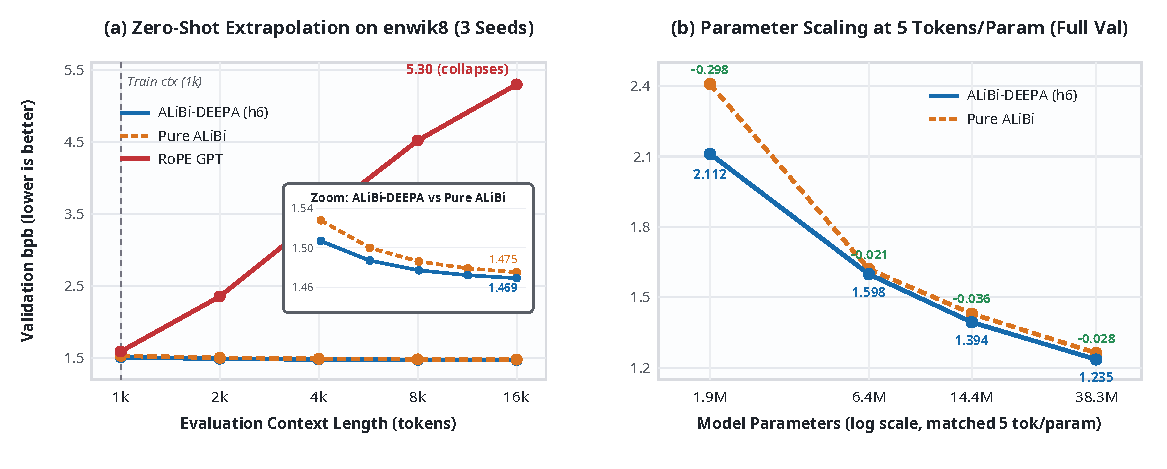
\includegraphics[width=\textwidth]{figs/fig2_extrap_scaling.pdf}
  \caption{\textbf{(a)} 3-seed zero-shot length extrapolation on \texttt{enwik8} ($1\text{k}\to 16\text{k}$) with zoomed inset: both ALiBi-DEEPA and Pure ALiBi improve monotonically while RoPE GPT collapses immediately past position 1,024. \textbf{(b)} Matched $5$ tokens/param scaling curve ($1.85\text{M}\to 38.34\text{M}$, full 1 MB validation; negative $\Delta$ = DEEPA better).}
  \label{fig:extrap_scale}
\end{figure}

\begin{table}[htbp]
\centering
\caption{Zero-shot length extrapolation on \texttt{enwik8} (3 seeds, trained at $T=1024$, scored on the identical $512\text{ KB}$ validation budget at every length).}
\label{tab:extrap}
\fitwidth{%
\begin{tabular}{lccccc}
\toprule
\textbf{Model (3 seeds)} & \textbf{$L=1024$} & \textbf{$L=2048$} & \textbf{$L=4096$} & \textbf{$L=8192$} & \textbf{$L=16384$} \\
\midrule
\textbf{ALiBi-DEEPA 3:1 (h6)} & \textbf{1.507 $\pm$ .008} & \textbf{1.487 $\pm$ .009} & \textbf{1.477 $\pm$ .010} & \textbf{1.472 $\pm$ .010} & \textbf{1.469 $\pm$ .010} \\
\textbf{Pure ALiBi} & 1.528 $\pm$ .003 & 1.500 $\pm$ .004 & 1.486 $\pm$ .004 & 1.479 $\pm$ .004 & 1.475 $\pm$ .004 \\
\textbf{RoPE GPT} & 1.588 $\pm$ .012 & 2.352 $\pm$ .070 & 3.454 $\pm$ .187 & 4.519 $\pm$ .179 & 5.299 $\pm$ .156 \\
\bottomrule
\end{tabular}}
\end{table}

\noindent\textbf{Analysis of Table~\ref{tab:extrap}:} ALiBi-DEEPA improves monotonically to $16\times$ its training length on every seed ($1.507 \to 1.469$ bpb), whereas RoPE GPT collapses past position 1,024 (per-position bucket loss jumps from $1.52$ in $0\text{k}\text{--}1\text{k}$ to $3.16$ in $1\text{k}\text{--}2\text{k}$ and $6.56$ in $15\text{k}\text{--}16\text{k}$). Beyond $2\text{k}$, DEEPA's mean lead over Pure ALiBi ($-0.006$ to $-0.009$ bpb) lies within seed spread (seed 2 favors Pure ALiBi past $2\text{k}$). Thus, ALiBi-DEEPA matches Pure ALiBi's stable $16\times$ extrapolation while requiring $4\times$ less KV cache ($50.7$ vs.\ $201.3\text{ MB}$ at $16\text{k}$).

\subsection{Multi-Domain Generalization (8 Datasets)}
We evaluate DEEPA across six additional byte-level domains (each $40\text{ MB}$ train / $1\text{ MB}$ disjoint validation, 3 seeds, 1,500 steps) plus WikiText-103 (evaluated both at 1,500 steps and at $5$ tokens/param = 4,406 steps after a per-model LR sweep confirming $2\times 10^{-3}$ is optimal for both models). Table~\ref{tab:domains} and Figure~\ref{fig:domains} report full-validation results.

\begin{figure}[htbp]
  \centering
  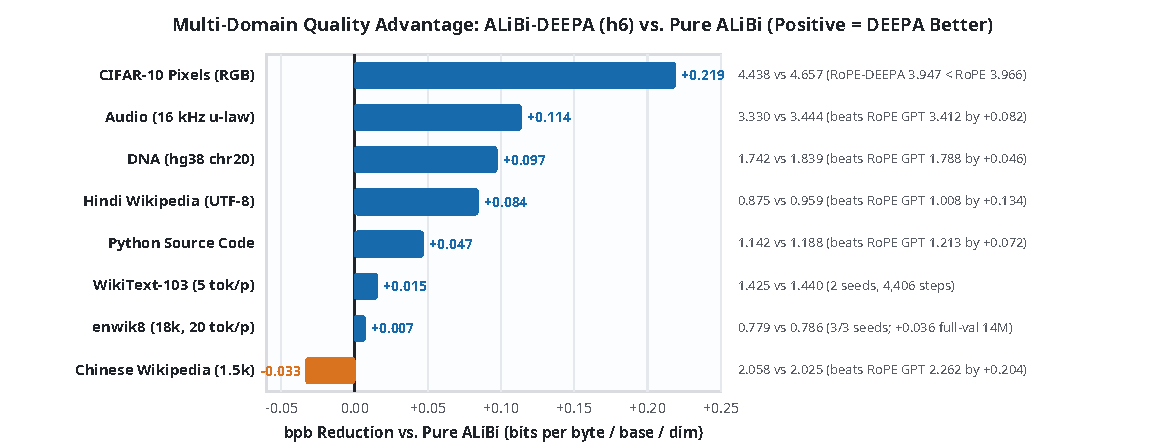
\includegraphics[width=\textwidth]{figs/fig3_multidomain.pdf}
  \caption{Multi-domain quality comparison of ALiBi-DEEPA (\texttt{h6}) vs.\ Pure ALiBi across all 8 real-world datasets. ALiBi-DEEPA beats Pure ALiBi on $7/8$ datasets; on CIFAR-10 pixels, swapping ALiBi for RoPE inside DEEPA (\texttt{RoPE-DEEPA}) beats RoPE GPT ($3.947$ vs.\ $3.966$ bpd).}
  \label{fig:domains}
\end{figure}

\begin{table}[htbp]
\centering
\caption{Multi-domain and multi-modal full-validation bpb (mean $\pm$ population std, 3 seeds unless noted; lower is better), including the Pure SheafDelta ($14.77\text{M}$, zero-attention) component ablation.}
\label{tab:domains}
\fitwidth{%
\begin{tabular}{lcccc}
\toprule
\textbf{Domain (Metric)} & \textbf{ALiBi-DEEPA (h6)} & \textbf{Pure ALiBi} & \textbf{RoPE GPT} & \textbf{Pure SheafDelta} \\
\midrule
\textbf{Python Source Code} (bpb) & \textbf{1.1416 $\pm$ .0057} & 1.1883 $\pm$ .0041 & 1.2131 $\pm$ .0075 & 1.3745 $\pm$ .0096 \\
\textbf{Hindi Wikipedia} (UTF-8) & \textbf{0.8745 $\pm$ .0016} & 0.9586 $\pm$ .0072 & 1.0081 $\pm$ .0261 & 0.8766 $\pm$ .0006 \\
\textbf{Chinese Wikipedia} (UTF-8) & 2.0581 $\pm$ .0069 & \textbf{2.0250 $\pm$ .0072} & 2.2617 $\pm$ .0071 & 2.0833 $\pm$ .0026 \\
\textbf{DNA, hg38 chr20} (bits/base) & 1.7420 $\pm$ .0002 & 1.8389 $\pm$ .0105 & 1.7881 $\pm$ .0020 & \textbf{1.7384 $\pm$ .0010} \\
\textbf{CIFAR-10 Pixels} (bits/dim) & 4.4382 $\pm$ .0136 & 4.6570 $\pm$ .0098 & \textbf{3.9661 $\pm$ .0084}$^\dagger$ & 4.4937 $\pm$ .0120 \\
\textbf{Speech 16 kHz $\mu$-law} (bps) & \textbf{3.3300 $\pm$ .0043} & 3.4436 $\pm$ .0112 & 3.4116 $\pm$ .0159 & 3.3311 $\pm$ .0056 \\
\midrule
\textbf{WikiText-103} (1.5k, 3s) & 1.6275 $\pm$ .0016 & \textbf{1.6154 $\pm$ .0020} & 1.7382 $\pm$ .0090 & --- \\
\textbf{WikiText-103} (4.4k, 2s) & \textbf{1.4250 $\pm$ .0017} & 1.4404 $\pm$ .0006 & --- & --- \\
\bottomrule
\multicolumn{5}{l}{\scriptsize $^\dagger$Diagnostic: \texttt{RoPE-DEEPA 3:1 (h6)} scores \textbf{3.9470 $\pm$ .0098} on CIFAR-10, beating RoPE GPT on $3/3$ seeds.}
\end{tabular}}
\end{table}

\noindent\textbf{Analysis of Table~\ref{tab:domains}:}
\begin{enumerate}
  \item \textbf{Multi-Modal Comparison \& Component Ablation:} ALiBi-DEEPA outperforms Pure ALiBi on $5/6$ new domains (Python code $-0.047$, Hindi $-0.084$, DNA $-0.097$, CIFAR-10 $-0.219$, Audio $-0.114$). Against Pure SheafDelta ($14.77\text{M}$, zero attention), ALiBi-DEEPA achieves 3 clear wins (Python code $-0.233$, Chinese $-0.025$, CIFAR-10 $-0.056$), 2 ties within $\sim 1\sigma$ (Hindi $0.8745$ vs.\ $0.8766$; Audio $3.3300$ vs.\ $3.3311$), and 1 loss on DNA ($1.7420$ vs.\ $1.7384$). The large code gap ($-0.233$ bpb) justifies keeping two attention layers for long-range identifier retrieval, while Pure SheafDelta's DNA win shows that a constant-memory ($0.49\text{ MB}$) model can outperform Transformers on genomics.
  \item \textbf{WikiText-103 Horizon Effect:} At 1,500 steps, Pure ALiBi led WikiText-103 by $0.012$ bpb; after verifying $2\times 10^{-3}$ is optimal for both models and training to $5$ tokens/param (4,406 steps), ALiBi-DEEPA leads on both seeds ($1.4250$ vs.\ $1.4404$ bpb, $-0.0154$) and at every evaluation length ($1\text{k}, 2\text{k}, 4\text{k}$). Chinese (at 1,500 steps) remains the sole domain where Pure ALiBi leads ALiBi-DEEPA ($2.025$ vs.\ $2.058$, while DEEPA beats RoPE GPT by $0.204$ bpb).
  \item \textbf{Causal Evidence on the CIFAR-10 Image Gap:} In row-major $32\times 32\times 3$ RGB bytes, the pixel directly above sits $96$ bytes back. ALiBi's monotonic distance penalty ($-m_h\cdot 96$) suppresses attention to that row for both ALiBi models. Swapping ALiBi for RoPE inside the \emph{same} DEEPA backbone (\texttt{RoPE-DEEPA}) recovers the entire $0.47$ gap and beats RoPE GPT on $3/3$ seeds ($3.9470 \pm .0098$ vs.\ $3.9661 \pm .0084$), showing that the limitation belongs to ALiBi's monotonic penalty on 2D strides rather than the Sheaf-Delta mixer. On Python code, \texttt{RoPE-DEEPA} ($1.145$) ties \texttt{ALiBi-DEEPA} ($1.142$) and resists $4\times$ length collapse ($1.136$ vs.\ RoPE GPT's $3.000$) because $6/8$ layers carry no positional encoding.
\end{enumerate}

\subsection{Training Speed, Inference Decoding, and 8 GB Serving}
\label{sec:systems}
Tables~\ref{tab:train_speed} and~\ref{tab:decode_serve} (and Figure~\ref{fig:systems}) report measured latencies, memory, and 8 GB serving capacity using FlashAttention-folded ALiBi, preallocated KV caches, and CUDA graphs for every model.

\begin{figure}[htbp]
  \centering
  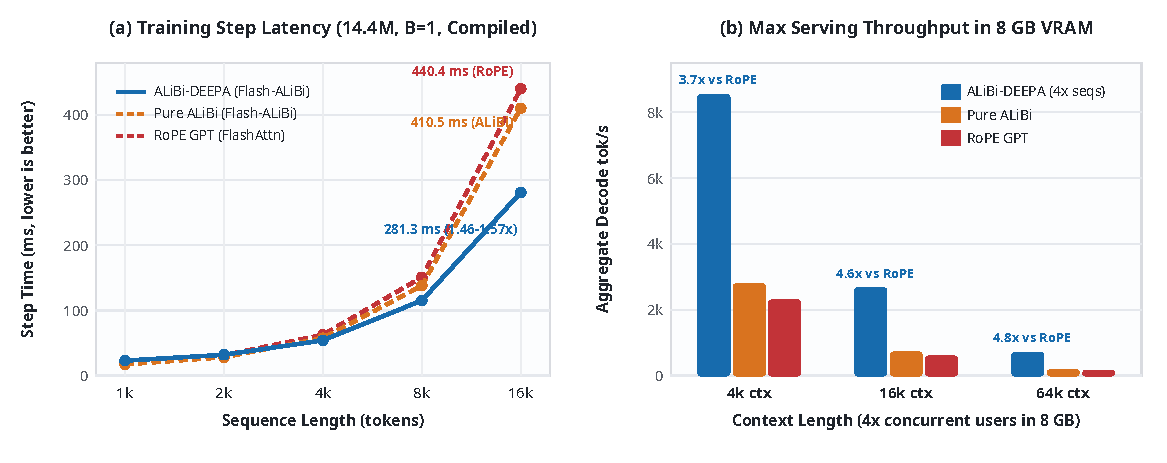
\includegraphics[width=\textwidth]{figs/fig4_systems_overhead.pdf}
  \caption{\textbf{(a)} Compiled training step latency ($14.4\text{M}, B=1$): with FlashAttention-folded ALiBi, DEEPA crosses below both RoPE GPT and Pure ALiBi between $2\text{k}$ and $4\text{k}$, running $1.46\text{--}1.57\times$ faster at $16\text{k}$. \textbf{(b)} Maximum aggregate decode throughput in 8 GB VRAM: DEEPA fits $4\times$ more concurrent users and achieves $3.7\text{--}4.8\times$ higher throughput than RoPE GPT ($3.1\text{--}4.2\times$ vs.\ Pure ALiBi).}
  \label{fig:systems}
\end{figure}

\begin{table}[htbp]
\centering
\caption{Compiled training step latency ($B=1$, no checkpointing), prefill latency, and peak training VRAM across sequence lengths ($14.4\text{M}$, FlashAttention-folded ALiBi for both DEEPA and Pure ALiBi vs.\ FlashAttention RoPE GPT).}
\label{tab:train_speed}
\fitwidth{%
\begin{tabular}{rcccccccc}
\toprule
\textbf{Length $T$} & \textbf{DEEPA Tr.} & \textbf{ALiBi Tr.} & \textbf{RoPE Tr.} & \textbf{DEEPA Pre.} & \textbf{ALiBi Pre.} & \textbf{RoPE Pre.} & \textbf{DEEPA MB} & \textbf{ALiBi / RoPE MB} \\
\midrule
1,024 & 22.8 ms & \textbf{17.0 ms} & 18.3 ms & 5.0 ms & \textbf{2.8 ms} & 3.6 ms & 414.8 & \textbf{349.4} / 359.2 \\
2,048 & 31.8 ms & \textbf{28.1 ms} & 31.1 ms & 6.3 ms & \textbf{5.8 ms} & 8.6 ms & 543.1 & \textbf{482.6} / 494.9 \\
4,096 & \textbf{54.0 ms} & 57.4 ms & 62.5 ms & \textbf{14.5 ms} & 15.6 ms & 18.7 ms & 855.9 & \textbf{746.7} / 774.7 \\
8,192 & \textbf{115.2 ms} & 137.9 ms & 150.9 ms & \textbf{31.2 ms} & 42.8 ms & 46.4 ms & 1,487.4 & \textbf{1,263.2} / 1,324.3 \\
16,384 & \textbf{281.3 ms} & 410.5 ms & 440.4 ms & \textbf{76.6 ms} & 125.1 ms & 135.0 ms & 2,749.3 & \textbf{2,283.8} / 2,408.6 \\
\bottomrule
\end{tabular}}
\end{table}

\begin{table}[htbp]
\centering
\caption{CUDA-graph autoregressive decoding latency (ms/token, best ALiBi implementation per regime: folded kernel at $B=1$, dense-mask path at $B=32$) and maximum 8 GB GPU serving capacity.}
\label{tab:decode_serve}
\fitwidth{%
\begin{tabular}{rrcccccc}
\toprule
\textbf{Context} & \textbf{Batch} & \textbf{DEEPA (ms)} & \textbf{Pure ALiBi} & \textbf{RoPE GPT} & \textbf{DEEPA 8 GB Cap.} & \textbf{ALiBi 8 GB Cap.} & \textbf{RoPE 8 GB Cap.} \\
\midrule
1,024 & 1 / 32 & 0.90 / \textbf{2.16} & \textbf{0.68} / 3.33 & 0.89 / 4.23 & --- & --- & --- \\
4,096 & 1 / 32 & \textbf{0.95} / \textbf{4.11} & 0.95 / 12.18 & 1.09 / 14.34 & \textbf{576 seq, 8,537 tok/s} & 144 seq, 2,781 tok/s & 144 seq, 2,283 tok/s \\
16,384 & 1 / 32 & \textbf{1.22} / \textbf{12.71} & 1.91 / 46.75 & 1.91 / 56.05 & \textbf{144 seq, 2,653 tok/s} & 36 seq, 700 tok/s & 36 seq, 578 tok/s \\
65,536 & 1 / 32 & \textbf{2.19} / \textbf{47.47} & 6.01 / OOM & 5.51 / OOM & \textbf{36 seq, 688 tok/s} & 9 seq, 163 tok/s & 9 seq, 144 tok/s \\
\bottomrule
\end{tabular}}
\end{table}

\noindent\textbf{Analysis of Tables~\ref{tab:train_speed} and~\ref{tab:decode_serve}:} With FlashAttention-folded ALiBi applied identically to DEEPA and Pure ALiBi, DEEPA surpasses FlashAttention RoPE GPT in prefill from $2\text{k}$ upward ($1.37\text{--}1.76\times$ faster) and in training from $4\text{k}$ upward ($1.16\text{--}1.57\times$ faster); against folded-kernel Pure ALiBi, DEEPA is slower at $1\text{k}\text{--}2\text{k}$ ($22.8$ vs.\ $17.0\text{ ms}$; $31.8$ vs.\ $28.1\text{ ms}$) and faster from $4\text{k}$ upward ($1.06\times$ at $4\text{k}$, $1.20\times$ at $8\text{k}$, $1.46\times$ at $16\text{k}$). In decoding, DEEPA is $2.0\text{--}4.4\times$ faster than RoPE GPT ($1.5\text{--}3.7\times$ faster than Pure ALiBi) at batch 32 across every length, $2.5\times$ faster at batch 1 at $64\text{k}$, and supports $4\times$ more concurrent users in $8\text{ GB}$---delivering $3.7\text{--}4.8\times$ higher aggregate throughput than RoPE GPT ($3.1\text{--}4.2\times$ higher than Pure ALiBi). At the $B=16, T=1024$ training recipe, small-kernel overhead makes DEEPA $\sim 26\%$ slower than folded-kernel Pure ALiBi ($86.5\text{k}$ vs.\ $117.0\text{k}$ tok/s) and $\sim 12\%$ slower than RoPE GPT ($98.5\text{k}$ tok/s); at $16\text{k}$, training VRAM is $14\%$ higher than RoPE GPT ($20\%$ higher than Pure ALiBi); and per-block activation checkpointing carries a $2.2\text{--}3.7\times$ recompute penalty on DEEPA vs.\ $1.0\text{--}1.3\times$ on attention models.

\subsection{Architectural Ablations and Falsified Design Variants}
\label{sec:ablation}
Table~\ref{tab:ablation} consolidates our 3-seed mixer-internal ablations (24 compiled runs on \texttt{enwik8}).

\begin{table}[htbp]
\centering
\caption{3-seed mixer-internal ablations ($1,500$ steps, \texttt{enwik8} 64 KB slice): \texttt{h6} is adopted for matched quality, $4.7\times$ tighter seed variance, and higher throughput.}
\label{tab:ablation}
\fitwidth{%
\begin{tabular}{lccccc}
\toprule
\textbf{Variant (3 seeds each)} & \textbf{Val @1024} & \textbf{@2048} & \textbf{@4096} & \textbf{tok/s} & \textbf{Verdict} \\
\midrule
v1 ALiBi-DEEPA ($H_{\text{mix}}=8, d_h=48$) & \textbf{1.0273 $\pm$ .0076} & \textbf{1.0067 $\pm$ .0066} & \textbf{1.0831 $\pm$ .0050} & 78.5k & Baseline \\
\textbf{\texttt{h6} ($H_{\text{mix}}=6, d_h=64$)} & \textbf{1.0291 $\pm$ .0016} & \textbf{1.0092 $\pm$ .0022} & \textbf{1.0869 $\pm$ .0057} & \textbf{80.7k} & \textbf{Adopt ($4.7\times$ tighter std)} \\
\texttt{decay} (\texttt{linspace(-1, 4.5)}) & 1.0452 $\pm$ .0091 & 1.0257 $\pm$ .0103 & 1.1037 $\pm$ .0113 & 75.4k & Reject ($+0.018$) \\
\texttt{h6\_postnorm\_scaled} & 1.0587 $\pm$ .0069 & 1.0401 $\pm$ .0069 & 1.1173 $\pm$ .0083 & 82.0k & Reject ($+0.030$) \\
\texttt{postnorm} (unscaled) & 1.0715 $\pm$ .0148 & 1.0539 $\pm$ .0163 & 1.1306 $\pm$ .0217 & 74.5k & Reject ($+0.044$) \\
\texttt{h6\_token\_shift} ($q,k$ shift) & 1.0751 $\pm$ .0103 & 1.0566 $\pm$ .0099 & 1.1317 $\pm$ .0059 & 77.6k & Reject ($+0.046$) \\
\bottomrule
\end{tabular}}
\end{table}

\noindent\textbf{Summary of Ablations:}
(1) Decoupling $H_{\text{mix}}=6$ ($d_h=64$) matches v1 quality while cutting seed variance $4.7\times$, accelerating training $+2.8\%$, and saving $109\text{ MB}$ VRAM.
(2) Both unscaled and $\sqrt{d_h}$-compensated post-sum normalization hurt by $+0.030$--$0.044$ bpb, confirming independent \texttt{onorm} on $o^{\text{delta}}$ is essential.
(3) Causal $q,k$ token-shift degrades loss by $+0.046$ bpb because blending $k_t + \alpha k_{t-1}$ before L2 normalization makes consecutive unit keys collinear, causing step $t$'s Householder erasure to overwrite step $t-1$.
(4) Re-initializing decay biases via \texttt{linspace(-1, 4.5)} pushes most heads to short $4$--$33$-token half-lives, duplicating the dyadic lags while starving long-range memory.
(5) Additional falsified designs: $4:1$ dilution (\texttt{ddddadddda}, $1.042$ bpb despite $+25\%$ params), sub-context SWA-512 ($1.061$ bpb), NoPE ($2.344$ bpb), low-rank MLPs ($+0.034$--$0.057$ bpb), and non-backprop credit assignment (DAD, DFA, layer-wise targets, JVP gradients).

\subsection{Long Range Arena, Causal $\beta$ Control, and Converged Synthetic Suite}
Tables~\ref{tab:lra}, \ref{tab:beta}, and~\ref{tab:synth} evaluate long-range classification (Long Range Arena \cite{tay2021}), the causal effect of negative eigenvalues ($\beta \in (0,1)$ vs.\ $(0,2)$), and a 9-task converged synthetic capability suite.

\begin{table}[htbp]
\centering
\caption{Long Range Arena \cite{tay2021} test accuracy ($D=256, L=4, 5{,}000$ steps, $B=32$, mean $\pm$ population std over 2 seeds).}
\label{tab:lra}
\begin{tabular}{lccc}
\toprule
\textbf{LRA Task} & \textbf{ALiBi-DEEPA (h6)} & \textbf{Pure ALiBi} & \textbf{RoPE GPT} \\
\midrule
ListOps ($\le 2\text{k}$) & 19.9 $\pm$ 0.3\% & 19.4 $\pm$ 0.6\% & 18.2 $\pm$ 0.3\% \\
IMDb bytes ($4\text{k}$) & \textbf{75.8 $\pm$ 0.3\%} & 63.7 $\pm$ 0.1\% & 54.6 $\pm$ 3.1\% \\
sCIFAR grayscale ($1\text{k}$) & \textbf{39.6 $\pm$ 0.1\%} & 36.8 $\pm$ 0.5\% & 34.9 $\pm$ 0.9\% \\
\bottomrule
\end{tabular}
\end{table}

\begin{table}[htbp]
\centering
\caption{Causal parity control ($D=128, L=4$, curriculum $8\to 64$, up to 20k steps, 3 seeds, identical parameter counts): capping $\beta \in (0,1)$ removes negative eigenvalues.}
\label{tab:beta}
\fitwidth{%
\begin{tabular}{lccc}
\toprule
\textbf{Model / $\beta$ Regime} & \textbf{Acc @64 (Train)} & \textbf{Acc @256 ($4\times$)} & \textbf{Steps to Solve} \\
\midrule
ALiBi-DEEPA, $\beta \in (0,1)$ & 99.9 / 99.3 / 99.8\% & 66.4 / 64.5 / 63.7\% & 11.5k / 12.5k / 12.5k \\
Pure SheafDelta, $\beta \in (0,1)$ & 99.8 / 99.9 / 99.6\% & 64.2 / 64.4 / 64.2\% & 11.5k / 11.0k / 17.5k \\
\textbf{ALiBi-DEEPA, $\beta \in (0,2)$} & \textbf{100 / 100 / 100\%} & \textbf{90.2 / 86.6 / 90.5\%} & \textbf{2.0k / 2.0k / 2.0k} \\
\textbf{Pure SheafDelta, $\beta \in (0,2)$} & \textbf{100 / 100 / 100\%} & \textbf{93.0 / 80.6 / 98.8\%} & \textbf{2.0k / 2.0k / 2.0k} \\
\bottomrule
\end{tabular}}
\end{table}

\begin{sidewaystable}
\centering
\caption{Converged synthetic capability suite ($D=128, L=4$ [1 attention layer in hybrid], except \texttt{Copy\_paper} which uses the paper $14.4\text{M}$ [$D=384, L=8$] model; up to 20k steps, LR grid, 3 seeds; accuracy \% per seed, `[steps]', `x' = unsolved).}
\label{tab:synth}
\fitwidth{%
\begin{tabular}{lllll}
\toprule
\textbf{Task} & \textbf{ALiBi-DEEPA 3:1 (Ours)} & \textbf{Pure ALiBi} & \textbf{RoPE GPT} & \textbf{Pure SheafDelta} \\
\midrule
\textbf{MQAR-8} ($T64$) \cite{arora2023} & \textbf{100/100/100 [1.5--3.5k]} & 99/99/100 [6--9k] & 99/100/99 [9--9.5k] & 99/99/100 [2.5--13.5k] \\
\textbf{MQAR-32} ($T512$) & \textbf{100/100/100 [2.5k all]} & 100/100/100 [3--6.5k] & 9/9/8 [x] & 100/99/100 [4.5--6k] \\
\textbf{MQAR-64} ($T512$) & 100/100/6 [4.5--6k] & 100/6/100 [3.5--9k] & 6/6/6 [x] & 100/6/100 [10k] \\
\textbf{Parity} ($64\to 256$) & \textbf{100$\to$90/87/90 [2k]} & 46--57$\to$31--52 [x] & 54--56$\to$44--52 [x] & \textbf{100$\to$93/81/99 [2k]} \\
\textbf{$S_3$ Group} ($64\to 256$) & \textbf{99--100$\to$93/95/48 [4--13k]} & 29--30$\to$20/20/20 [x] & 28$\to$20/20/19 [x] & \textbf{99--100$\to$92/89/96 [2.5--6k]} \\
\textbf{$S_5$ Group} ($64\to 256$) & 4/2/3$\to$2/1/1 [x] & 2/2/2$\to$1/1/1 [x] & 2/2/2$\to$1/1/1 [x] & 4/6/6$\to$2/2/2 [x] \\
\textbf{Copy\_paper} ($128\to 512$) \cite{jelassi2024} & 100$\to$100/98/38 [2--4k] & \textbf{100$\to$96/95/87 [0.5k]} & 100$\to$0/0/0 [0.5k] & 99--100$\to$14/18/15 \\
\textbf{Copy} ($128\to 512$) & 100/2/100$\to$96/0/59 & \textbf{100$\to$99/98/99 [1k]} & 100$\to$0/0/0 [0.5k] & 99$\to$24/26/19 \\
\textbf{SelCopy} ($T256$) & 99/99/99 [3.5--10.5k] & 100/99/99 [7--10k] & 99/100/99 [4--6.5k] & \textbf{100/100/99 [3--4k]} \\
\bottomrule
\end{tabular}}
\end{sidewaystable}

\noindent\textbf{Analysis of Tables~\ref{tab:lra}--\ref{tab:synth}:}
(1) \textbf{Long Range Arena:} ALiBi-DEEPA achieves 2 clear wins---beating Pure ALiBi by $+12.1\%$ and RoPE GPT by $+21.2\%$ on 4k-byte IMDb ($75.8\%$ vs.\ $63.7\%$ / $54.6\%$), and winning sCIFAR ($39.6\%$ vs.\ $36.8\%$ / $34.9\%$)---and ties within noise at chance on ListOps ($19.9 \pm 0.3\%$ vs.\ $19.4 \pm 0.6\%$).
(2) \textbf{Causal Evidence for Negative Eigenvalues:} Capping $\beta \in (0,1)$ slows parity convergence $5.5\text{--}8.7\times$ ($2\text{k}\to 11\text{--}17.5\text{k}$ steps) and drops $4\times$ length extrapolation from $\sim 90\%$ down to $\sim 64\%$ on both mixers, providing direct causal evidence that $\beta \in (0,2)$ drives length-general state tracking.
(3) \textbf{Capability Coverage \& LR Robustness:} ALiBi-DEEPA 3:1 is the only model with non-trivial success across all three capability families: associative recall (fastest on MQAR-8 and MQAR-32), state tracking (parity and non-abelian $S_3$, where Pure ALiBi and RoPE GPT fail), and length-general copying (\texttt{Copy\_paper}, where RoPE [$0\%$] and Pure SheafDelta [$14\text{--}18\%$] collapse). A full learning-rate robustness grid (every LR evaluated on all 3 seeds, selecting each model's LR by 3-seed mean) clarifies two points: first, the earlier small-model copy failure came from selecting $\text{LR}=3\times 10^{-3}$ via seed 0 alone---at its mean-optimal LR, DEEPA solves both \texttt{Copy\_paper} ($3/3$ at $10^{-3}$, $79\%$ mean at $4\times$) and small \texttt{Copy} ($3/3$ at $3\times 10^{-4}$, $33\%$ at $4\times$) on every seed, though Pure ALiBi still copies substantially better at $4\times$ ($93\text{--}100\%$) and $4\times$ faster. Second, on MQAR-64 at a single fixed LR, DEEPA solves $2/3$ seeds (the remaining seed reaches $94\%$), whereas Pure ALiBi ($3/3$) and Pure SheafDelta ($3/3$) reach $3/3$ (RoPE $0/3$). All four models fail $NC^1$-complete $S_5$ \cite{merrill2024}.

% ======================== SECTION 6 ========================
\section{Limitations and Future Work}

We note six concrete boundaries of this study:
\begin{enumerate}
  \item \textbf{Short-Context Kernel Overhead ($T \le 1\text{k}$):} At $B=16, T=1024$, small-kernel launch overhead in the 6 Sheaf-Delta layers makes DEEPA $\sim 26\%$ slower than folded-kernel Pure ALiBi ($86.5\text{k}$ vs.\ $117.0\text{k}$ tok/s) and $\sim 12\%$ slower than RoPE GPT ($98.5\text{k}$ tok/s), while using $14\%$ more training VRAM at $16\text{k}$ than RoPE GPT ($2{,}749$ vs.\ $2{,}409\text{ MB}$) and $20\%$ more than folded-kernel Pure ALiBi ($2{,}284\text{ MB}$). Fusing the Householder dyadic transport and output projection into a single Triton kernel is the primary systems next step.
  \item \textbf{Monotonic ALiBi Penalty on 2D Raster Strides:} As shown by our CIFAR-10 \texttt{RoPE-DEEPA} diagnostic ($3.947$ vs.\ \texttt{ALiBi-DEEPA} $4.438$ bpd), ALiBi's monotonic distance decay handicaps fixed long-stride 2D dependencies. Mixing zero-slope or weak-slope heads in the attention layers is a targeted extension for 2D modalities.
  \item \textbf{Copying Extrapolation and MQAR-64 Reliability:} Although DEEPA solves exact copying on $3/3$ seeds at trained length under its mean-optimal LR, it learns copying $4\times$ slower than Pure ALiBi and trails Pure ALiBi at $4\times$ length ($79\%$ paper / $33\%$ small vs.\ $93\text{--}100\%$). On MQAR-64 at a single LR, DEEPA solves $2/3$ seeds (the remaining seed reaches $94\%$) vs.\ $3/3$ for Pure ALiBi and Pure SheafDelta.
  \item \textbf{Unsolved $S_5$ and Chance-Level ListOps:} All four single-step models fail $NC^1$-complete $S_5$ state tracking (motivating multi-reflection products \cite{siems2025} as future work), and all models remain near chance on LRA ListOps at this budget.
  \item \textbf{Byte-Level Scope Only:} All experiments are byte-level ($V=256$); subword (BPE) pretraining and downstream zero-shot benchmarks remain to be evaluated.
  \item \textbf{Scale Beyond $38\text{M}$ Converged Parameters:} While our scaling law validates DEEPA from $1.85\text{M}$ to $38.34\text{M}$ parameters at $5$ tokens/param (and VRAM fits $206\text{M}$ in $5.3\text{ GB}$), full Chinchilla training at $100\text{M}\text{--}1\text{B}$ scale on multi-GPU clusters remains future work.
\end{enumerate}

% ======================== SECTION 7 ========================
\section{Conclusion}

We presented \textbf{DEEPA} (\textbf{D}yadic-Delta \textbf{E}nhanced-sheaf, \textbf{E}fficient \textbf{P}airing with \textbf{A}LiBi), a $3:1$ hybrid sequence model pairing negative-eigenvalue gated delta-rule matrix memory and parallel isometric dyadic sheaf diffusion with FlashAttention-folded ALiBi attention. Across 8 diverse real-world datasets, 4 parameter scales ($1.85\text{M}\to 38.34\text{M}$), 18,000-step and equal-wall-clock convergence, 3-seed $16\times$ extrapolation, Long Range Arena ($2/3$ clear wins, $1$ tie at chance), and a 9-task converged synthetic suite, ALiBi-DEEPA outperforms Pure ALiBi on $7/8$ domains and all 4 parameter scales, achieves 3 wins, 2 ties, and 1 loss against Pure SheafDelta across 6 domains, is the sole model with non-trivial success across recall, parity/$S_3$ state tracking, and $4\times$ copying, cuts inference KV cache by $4\times$, increases 8 GB serving throughput by $3.7\text{--}4.8\times$ vs.\ RoPE GPT ($3.1\text{--}4.2\times$ vs.\ Pure ALiBi), and accelerates $4\text{k}\text{--}16\text{k}$ training by $1.16\text{--}1.57\times$ over FlashAttention RoPE GPT ($1.06\text{--}1.46\times$ over folded-kernel Pure ALiBi).

% ======================== SPRINGER DECLARATIONS ========================
\section*{Declarations}
\small
\noindent\textbf{Funding:} No external funding was received for conducting this study.\\
\noindent\textbf{Competing Interests:} The authors declare no competing financial or non-financial interests.\\
\noindent\textbf{Data Availability:} All datasets used in this study are publicly available (enwik8 \cite{hutter2006}, WikiText-103 \cite{merity2016}, CIFAR-10 \cite{krizhevsky2009}, GRCh38/hg38 \cite{grch38}, Speech Commands \cite{warden2018}, Wikipedia dumps, and CodeParrot \cite{codeparrot}).\\
\noindent\textbf{Code Availability:} Complete training scripts, Triton-fused kernels, and benchmark suites will be released publicly upon acceptance.

% ======================== REFERENCES ========================
\begin{thebibliography}{99}
\scriptsize
\bibitem{vaswani2017} Vaswani, A., Shazeer, N., Parmar, N., et al.: Attention is all you need. In: NeurIPS, vol.\ 30 (2017)
\bibitem{su2024} Su, J., Ahmed, M., Lu, Y., Pan, S., Bo, W., Liu, Y.: RoFormer: Enhanced Transformer with rotary position embedding. Neurocomputing 568, 127063 (2024)
\bibitem{press2022} Press, O., Smith, N.A., Lewis, M.: Train short, test long: Attention with linear biases enables input length extrapolation (ALiBi). In: ICLR (2022)
\bibitem{dao2022} Dao, T., Fu, D.Y., Ermon, S., Rudra, A., R\'e, C.: FlashAttention: Fast and memory-efficient exact attention with IO-awareness. In: NeurIPS, vol.\ 35, pp.\ 16344--16359 (2022)
\bibitem{katharopoulos2020} Katharopoulos, A., Vyas, A., Pappas, N., Fleuret, F.: Transformers are RNNs: Fast autoregressive transformers with linear attention. In: ICML, pp.\ 5156--5165 (2020)
\bibitem{schlag2021} Schlag, I., Irie, K., Schmidhuber, J.: Linear Transformers are secretly fast weight programmers. In: ICML, pp.\ 9355--9366 (2021)
\bibitem{gu2023} Gu, A., Dao, T.: Mamba: Linear-time sequence modeling with selective state spaces. In: COLM (2024)
\bibitem{dao2024} Dao, T., Gu, A.: Transformers are SSMs: Generalized models and efficient algorithms through structured state space duality (Mamba-2). In: ICML (2024)
\bibitem{yang2024b} Yang, S., Wang, B., Zhang, Y., Shen, Y., Kim, Y.: Parallelizing linear transformers with the delta rule over sequence length (DeltaNet). In: NeurIPS (2024)
\bibitem{yang2024c} Yang, S., Kautz, J., Hatamizadeh, A.: Gated Delta Networks: Improving Mamba2 with delta rule. In: ICLR (2025)
\bibitem{grazzi2024} Grazzi, R., Siems, J., Zela, A., Garg, S., Hutter, F., Pontil, M.: Unlocking state-tracking in linear RNNs through negative eigenvalues. In: ICLR (2025)
\bibitem{siems2025} Siems, J., Carstensen, T., Zela, A., Hutter, F., Pontil, M., Grazzi, R.: DeltaProduct: Improving state-tracking in linear RNNs via Householder products. arXiv:2502.10297 (2025)
\bibitem{merrill2024} Merrill, W., Petty, J., Sabharwal, A.: The illusion of state in state-space models. In: ICML (2024)
\bibitem{bischof1987} Bischof, C., Van Loan, C.: The WY representation for products of Householder matrices. SIAM J.\ Sci.\ Stat.\ Comput.\ 8(1), s2--s13 (1987)
\bibitem{lieber2024} Lieber, O., Lenz, B., Bata, H., et al.: Jamba: A hybrid Transformer-Mamba language model. arXiv:2403.19887 (2024)
\bibitem{ren2024} Ren, L., Liu, Y., Lu, Y., et al.: Samba: Simple hybrid state space models for efficient unlimited context language modeling. arXiv:2406.07522 (2024)
\bibitem{waleffe2024} Waleffe, R., Byeon, W., Riach, D., et al.: An empirical study of Mamba-based language models. arXiv:2406.07887 (2024)
\bibitem{kazemnejad2023} Kazemnejad, A., Padhi, I., Natesan Ramamurthy, K., Das, P., Reddy, S.: The impact of positional encoding on length generalization in Transformers (NoPE). In: NeurIPS, vol.\ 36 (2023)
\bibitem{peng2023} Peng, B., Quesnelle, J., Fan, H., Shippole, E.: YaRN: Efficient context window extension of large language models. In: ICLR (2024)
\bibitem{hutter2006} Hutter, M.: The Human Knowledge Compression Prize (enwik8). \url{http://prize.hutter1.net/} (2006)
\bibitem{merity2016} Merity, S., Xiong, C., Bradbury, J., Socher, R.: Pointer sentinel mixture models (WikiText-103). In: ICLR (2017)
\bibitem{krizhevsky2009} Krizhevsky, A.: Learning multiple layers of features from tiny images (CIFAR-10). Tech.\ Rep., Univ.\ of Toronto (2009)
\bibitem{grch38} Schneider, V.A., Graves-Lindsay, T., Howe, K., et al.: Evaluation of GRCh38 and de novo haploid genome assemblies demonstrates the enduring quality of the reference assembly. Genome Res.\ 27(5), 849--864 (2017)
\bibitem{warden2018} Warden, P.: Speech Commands: A dataset for limited-vocabulary speech recognition. arXiv:1804.03209 (2018)
\bibitem{vandenoord2016} van den Oord, A., Dieleman, S., Zen, H., et al.: WaveNet: A generative model for raw audio. arXiv:1609.03499 (2016)
\bibitem{codeparrot} Tunstall, L., von Werra, L., Wolf, T.: CodeParrot: Clean Python code dataset. Hugging Face Hub (2022)
\bibitem{hoffmann2022} Hoffmann, J., Borgeaud, S., Mensch, A., et al.: Training compute-optimal large language models (Chinchilla). In: NeurIPS, vol.\ 35 (2022)
\bibitem{tay2021} Tay, Y., Dehghani, M., Abnar, S., et al.: Long Range Arena: A benchmark for efficient transformers. In: ICLR (2021)
\bibitem{arora2023} Arora, S., Eyuboglu, S., Timalsina, A., et al.: Zoology: Measuring and improving recall in efficient language models. In: ICLR (2024)
\bibitem{jelassi2024} Jelassi, S., Brandfonbrener, D., Kakade, S.M., Malach, E.: Repeat after me: Transformers are better than state space models at copying. In: ICML (2024)
\end{thebibliography}

\end{document}
